% !TeX encoding = UTF-8
% !TeX program = pdflatex

\documentclass[11pt]{article}
\usepackage{graphicx}

\newcommand\CIPH{C\!I\!P\!H_K}

\title{{\bf The usage and the impact of shift registers on the CFB mode of operation} \\ \bigskip \large HW1 - CNS Sapienza}
\date{2018-10-12}
\author{Andrea Fioraldi 1692419}
\pagenumbering{roman}

\begin{document}
\maketitle

\section{Introduction}

With the aim to provide confidentiality and authenticity of information, {\em Block Ciphers} are widely used in cryptography. Block Ciphers operates on fixed-length messages, called {\em blocks}, and {\em Modes of Operations} are the techniques used to apply block ciphers to messages longer than a block.

{\em Cipher Feed Back} (CFB) is a popular mode of operation.
In the following sections, we will discuss the usage and the impact of CFB and, in particular, of its variant that uses shift registers.

\section{CFB Overview}

\begin{figure}[!ht]
  \centering
  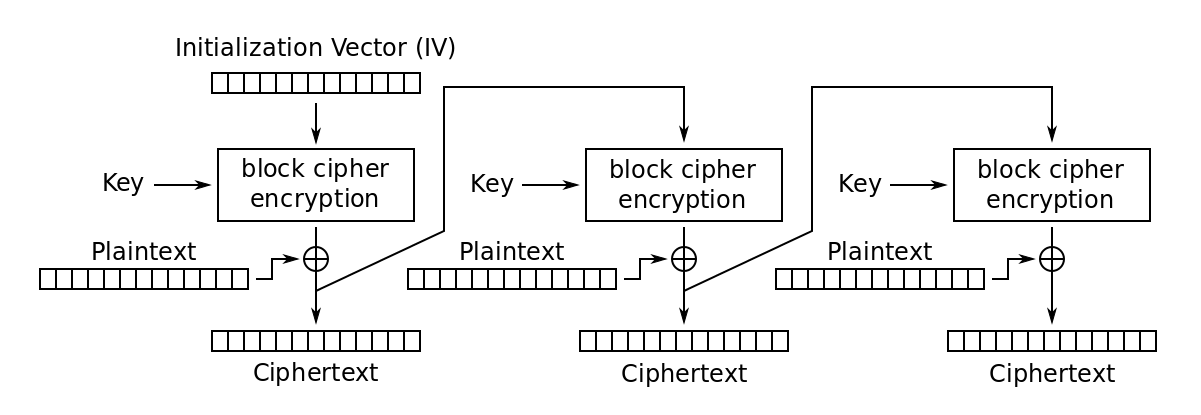
\includegraphics[width=1\textwidth]{pic1-hw1-1692419}
  \caption{CFB encryption, from \cite{wiki}}
  \label{fig:cfb_enc}
\end{figure}

In this technique, regards the encryption, the produced ciphertext block is forwarded to the next encryption unit to produce a block of encrypted data that, xored\footnote{exclusive-ORed} with the correspondent plaintext block, generates the next ciphertext block. 

\begin{figure}[!ht]
  \centering
  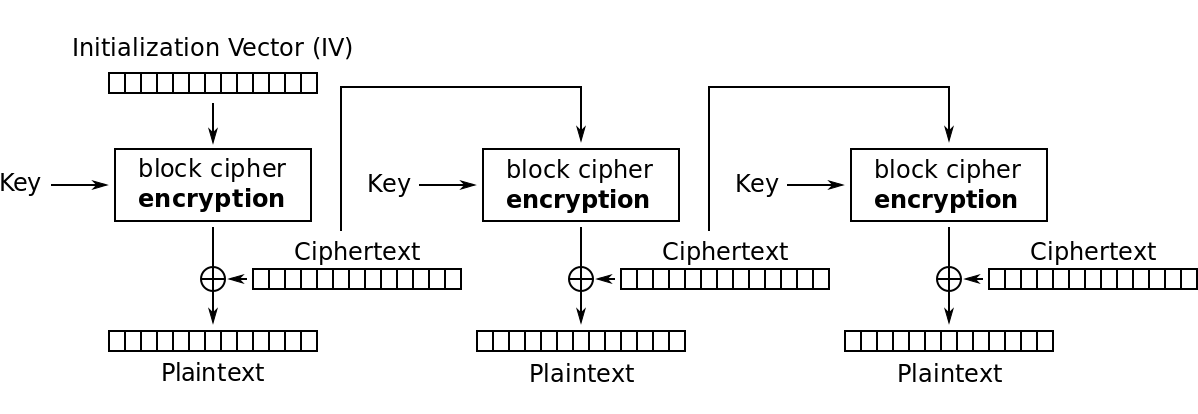
\includegraphics[width=1\textwidth]{pic2-hw1-1692419}
  \caption{CFB decryption, from \cite{wiki}}
  \label{fig:cfb_dec}
\end{figure}

Viceversa, during the decryption, the output of the encryption unit using the previous ciphertext block is xored with the current ciphertext block to produce the corresponding plaintext block.

This mode of operation requires an initialization vector (IV) as the initial input block. As you can see in figure \ref{fig:cfb_dec} the encryption unit is used also for decryption.

Accordingly to \cite{wiki}, CFB encryption and decryption can be expressed with the following formulas:

\begin{itemize}
\item Encryption: $C_0 = IV$, $C_i = \CIPH(C_{i-1}) \oplus P_i$ $\forall i = 1...n$;
\item Dencryption: $P_0 = IV$, $P_i = \CIPH(C_{i-1}) \oplus C_i$ $\forall i = 1...n$;
\end{itemize}

The used symbols are defined in the following way:

\begin{itemize}
\item $IV := $ the initialization vector;
\item $\CIPH := $ the encryption process using the key $K$;
\item $P_i := $ the i-th block of the plaintext;
\item $C_i := $ the i-th block of the ciphertext;
\item $n := $ number of blocks composing the plaintext/ciphertext;
\end{itemize}

An additional property is the possibility to use parallelism in the decryption process. 

CFB is an example of stream cipher, in fact the encryption is done one block at time and depends from the state. 

\section{CFB with Shift Registers}

One of the most used variants of CFB introduces shift registers as input for the encryption unit.

\subsection{Usage}

Before describing the usage of the shift registers in the CFB mode we must provide some additional definitions:

\begin{itemize}
\item $b := $ the size of a block in bits;
\item $s := $ the size of a plaintext/ciphertext segment in bits ($1 \le s \le b$);
\item $SR := $ the content of the input shift register;
\item $P_i := $ the i-th segment of the plaintext;
\item $C_i := $ the i-th segment of the ciphertext;
\end{itemize}

We define a {\em segment} as a block of the plaintext/ciphertext on which CFB operates. It can be smaller than the type of blocks used by $\CIPH$, so we use the term segment to distinguish between them.

\begin{figure}[!ht]
  \centering
  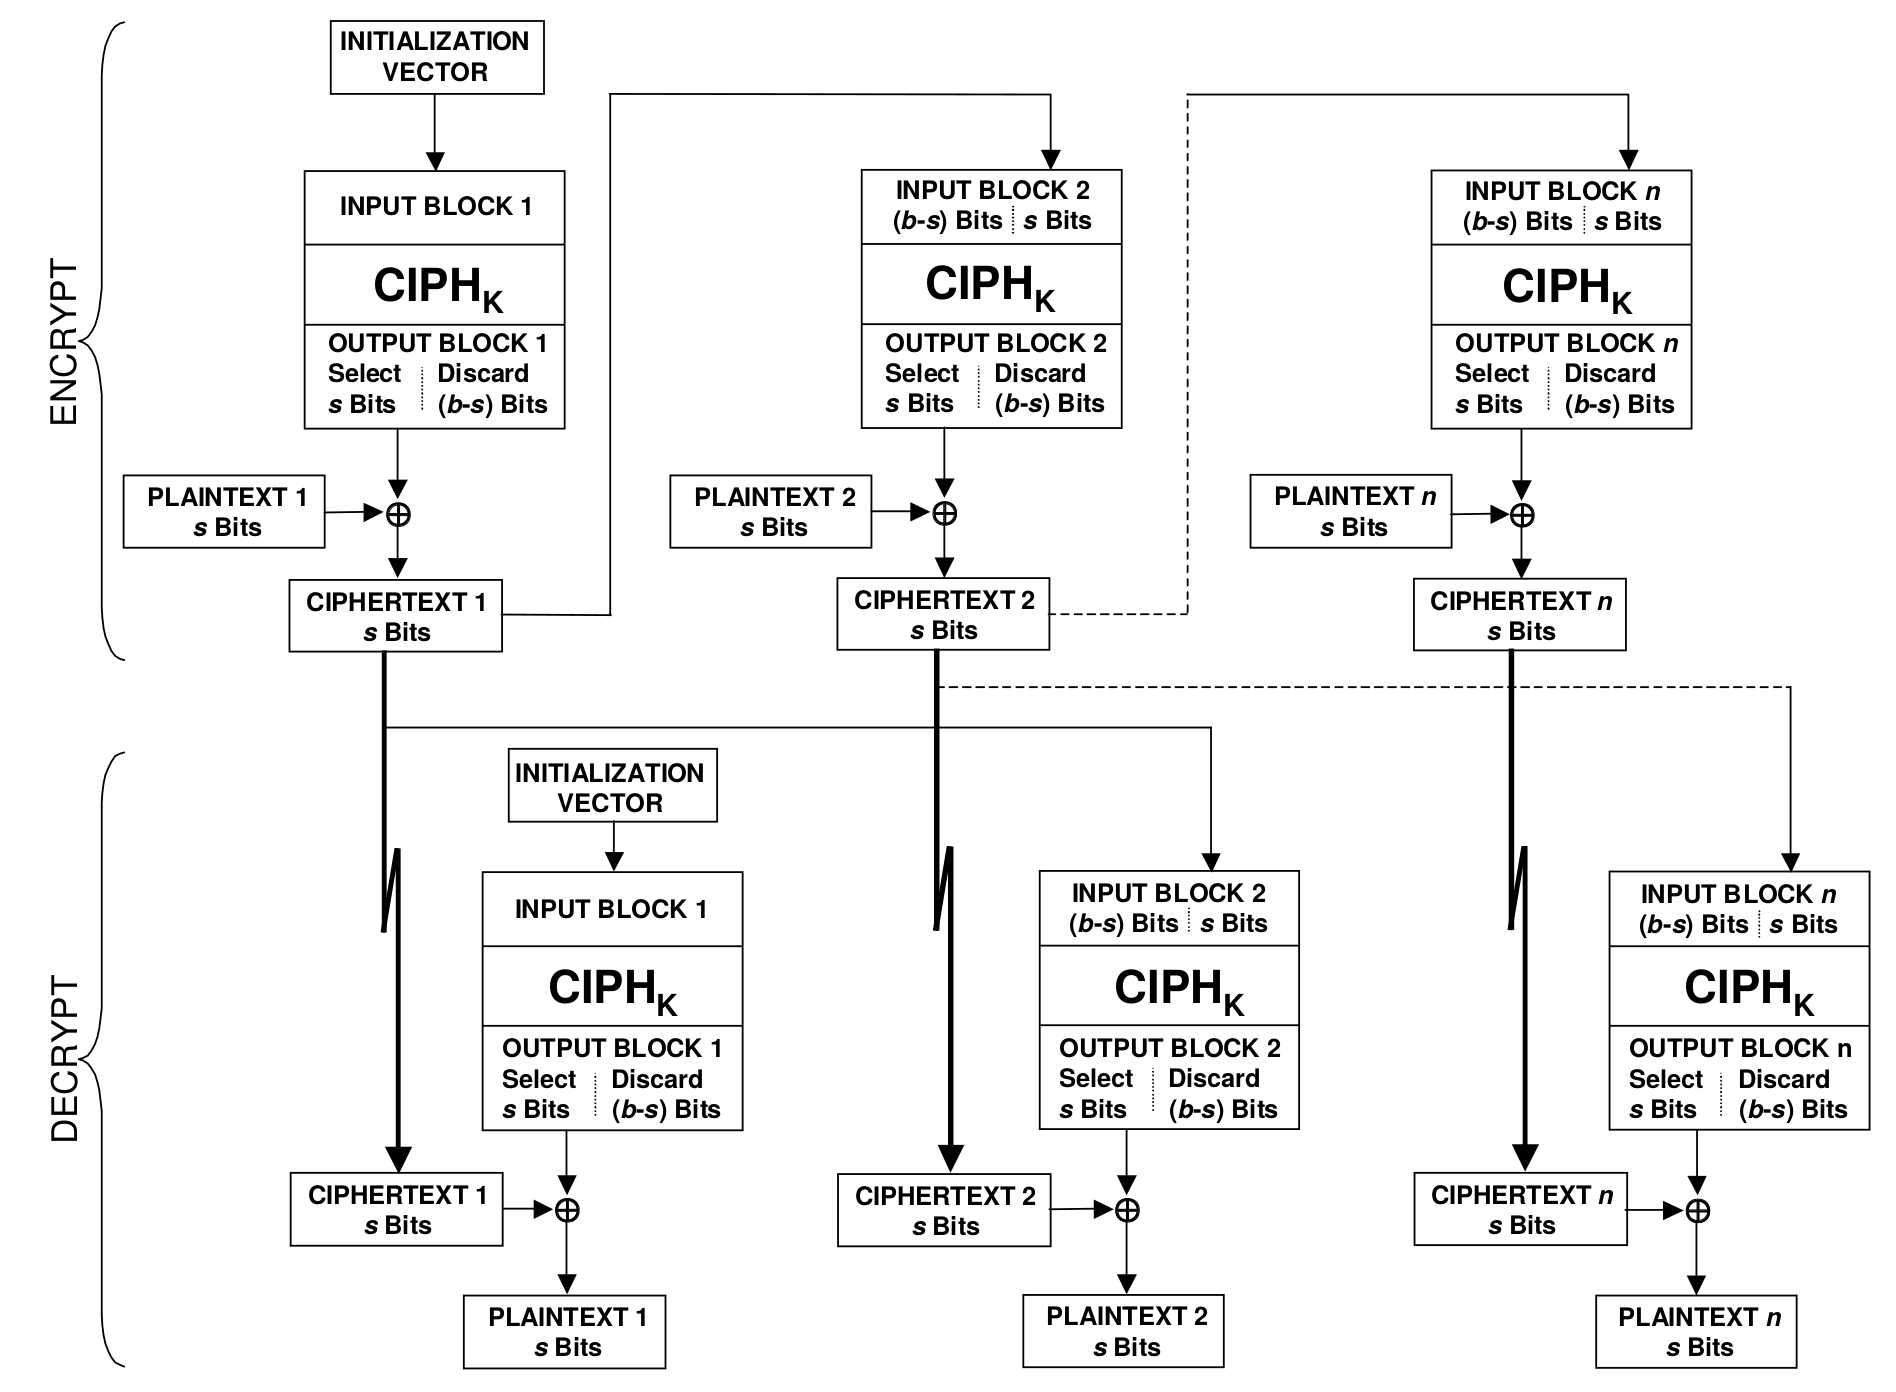
\includegraphics[width=1\textwidth]{pic3-hw1-1692419}
  \caption{CFB with shift registers, from \cite{nist}}
  \label{fig:cfb_shift}
\end{figure}

In this variant of the technique, only the $s$ most significant bits of the $E_K$ output are xored with the plaintext segment to produce a ciphertext segment. Then, to form the next input block, the $b - s$ least significant bits of the previous input block are shifted to left of $s$ positions and thus remaining space is filled with the $s$ bits of the previous ciphertext segment. The $IV$ is used as usual.
The decryption works in a similar way, the input ciphertext segment is placed in the input block after shifting the $b - s$ least significant bits.

The mathematical formulas for CFB with shift registers are the following:

\begin{itemize}
\item Encryption: $C_i = extract(E_K(SR_{i-1}), s) \oplus P_i$ $\forall i = 1...n$;
\item Dencryption: $P_i = extract(E_K(SR_{i-1}), s) \oplus C_i$ $\forall i = 1...n$;
\end{itemize}

Where $extract(x, y)$ are the most significant $y$ bits of a message $x$. The evolution of the content of $SR$ in both encryption and decryption is described by:

$S_0 = IV$, $S_i = ((S_{i-1} << s) + C_i)$ $mod$ $2^n$ $\forall i = 1...n$.

\subsection{Impact}

The usage of shift registers in CFB mode provides a significant property that is not present in the traditional technique: it makes the block cipher a self-synchronizing stream cipher. A cipher is called self-synchronizing when, if a part of the ciphertext is lost, the decryption can continue correctly after a finite number of incorrect decryptions of blocks.
In the standard CFB if a bit of the ciphertext is lost the technique is not able to synchronize.
With the shift registers, instead, if we lost $x$ bits of a ciphertext segment $C_j$, the decryption will produce wrong plaintext segments until that there are some bits of $C_j$ in $SR$. The number of the corrupted plaintext segments is $n/s$.

\section{Conslusion}

Introducing shift registers in the CFB mode is a game-changing choice with a low impact on performance. In fact, the implementations in software and in hardware are not more complicated than the standard technique and with a reasonable overhead of $b/s * n$ calls to $E_K$ versus the $n$ calls performed in the traditional CFB. 

\vfill

\begin{thebibliography}{99}

\bibitem{wiki}
{\em Block cipher mode of operation - Wikipedia}.
  \verb|https://en.wikipedia.org/wiki/Block_cipher_mode_of_operation|
  \newblock Accessed: 2018-10-12.

\bibitem{nist}
Morris Dworkin.
  {\em Recommendation for Block Cipher Modes of Operation. Methods and Techniques}.
  Tech. rep. 800-38A. National Institute of Standards and Technology, 2001.
  \newblock \verb|url: http://www.dtic.mil/docs/citations/ADA400014|

\end{thebibliography}

\end{document}
